After the panel factorization, the operation performed on the trailing sub-matrix is the update. The update takes the array of pivots produced by the panel factorization, swaps the rows and then apply \emph{trsm} and \emph{gemm} operations.

To perform one swap, the algorithm depends on the value of the pivots, this is what we call data dependency and so the algorithm is a dynamic algorithm (section \ref{task_flow_lu}). The solution to represent a dynamic algorithm with a static DAG of task flow is to make a path with all tasks. In practice, it means that all tiles must participate in swapping even if they are not concerned.
For that, each tile will have a workspace of two rows: the first to store one row coming from the upper tile and the second to store one row going to the upper tile. Nodes will share between them the workspaces and fill them with the appropriate rows.
The \emph{all\_reduce} seems to be the right operation to use. 
At the step $k$, $n_t-k$ tiles participate to the election of the best pivot. The cost of an \emph{all\_reduce} operation is $log_2$. Thus, a swap operation costs:
\begin{center}
$log_2(n_t-k)$
\end{center}
There is $n_b$ swaps per panel. Thus, the cost of all swaps of one panel is:
\begin{center}
$n_b*log_2(n_t-k)$
\end{center}.
The cost of swaps of all panel of one step $k$ is:
\begin{center}
$n_b*log_2(n_t-k)*(n_t-k)$
\end{center}.
Finally, the cost of all swaps of the LU decomposition is:
\begin{center}
$$\sum_{k=0}^{nt-1} n_b*log_2(n_t-k)*(n_t-k)$$
\end{center}.

In SPMD model, a single swap costs $2*n_b$. Thus, with the same reasoning, the cost of all swaps of the SPMD LU decomposition obtained is:
\begin{center}
$2*n_b*(n_t^2-n_t)/2$
\end{center}.

The natural task flow algorithm will be very expensive relatively to the cost of SPMD algorithm. Moreover, at the end of each \emph{all\_reduce} operation, only two nodes will really use the rows collected in their workspace (the upper tile and the tile which exchanges with it).

In order to reduce the cost of swaps, a good idea is to perform all swaps at the same time. However, this is not possible with pivots. In fact, because the same row can own several times the row including the maximum of the column, it is necessary to execute the pivots in the right order (from the first to the last). Figure \ref{fig:pivots} shows an example of a row which contains successively two times the maximum value of the column, we can see that the row 1 goes down to the row 13 then comes back to the row 2. Thus, it forces us to perform the first pivots before the second.

\begin{figure}[!ht]
\begin{minipage}[!ht]{.4\textwidth}
\centering
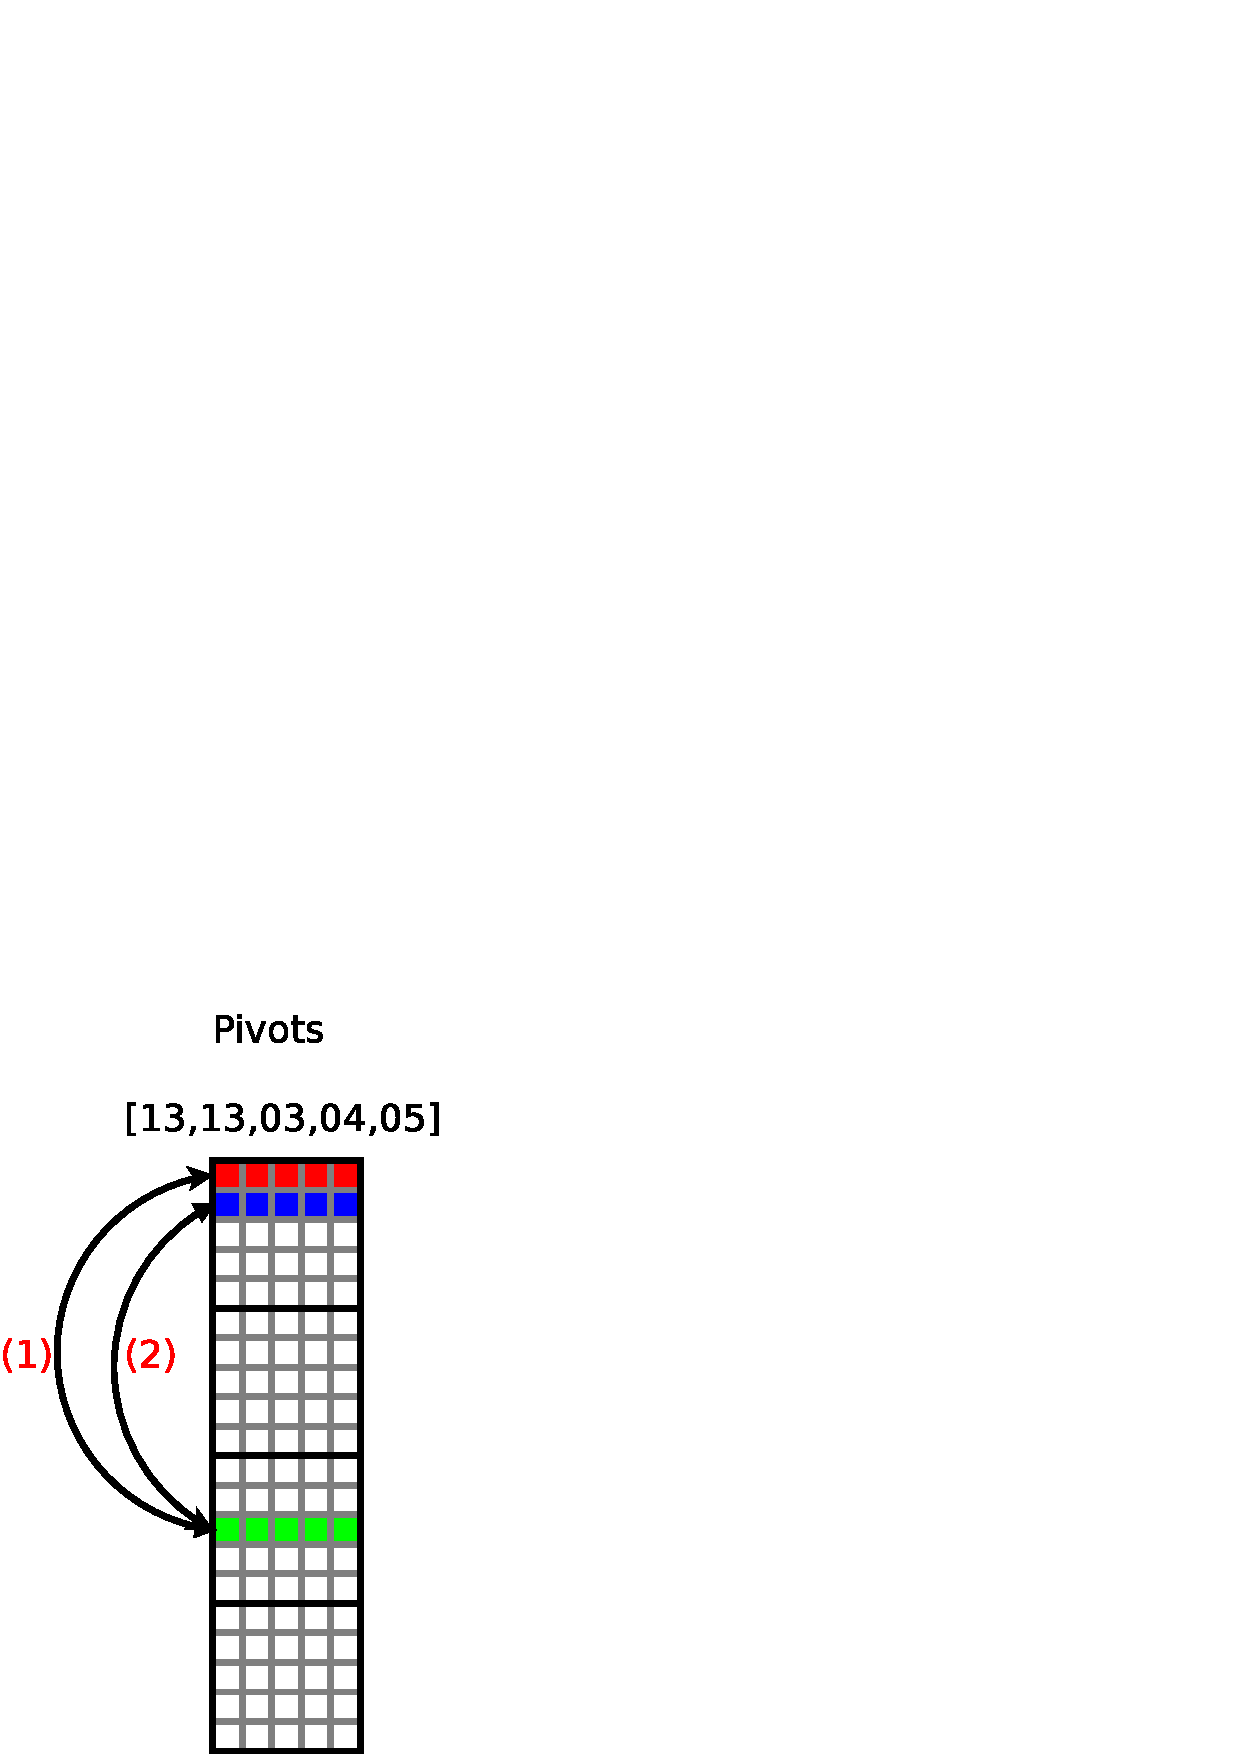
\includegraphics[height=5cm]{figures/pivots.pdf}
\caption{Row movements with pivots\label{fig:pivots}}
\end{minipage} \hfill
\begin{minipage}[!ht]{.4\textwidth}
\centering
\includegraphics[height=5cm]{figures/permutations.pdf}
\caption{Row movements with permutations\label{fig:permutations}}
\end{minipage}
\end{figure}

To reduce high cost of all swaps, the key is to use another structure instead of pivots. For that, the permutations are the right solution. In fact, permutations can be represented by an array of size $n$ (we see after that it can be reduced). For each index $x$ of the array $perm$, the row $perm(x)$ will be moved in place of the row $x$. Thus, with permutations, we know from the beginning the final place of each row. 
Figure \ref{fig:permutations} shows the use of permutations instead of pivots which is showed in Figure \ref{fig:pivots}, we can see that the row 1 goes directly to the row 2 and does	 not move again.
Thanks to this structure, all the rows of one panel can be swapped in one single step. Thus, the cost of all swaps of one panel will be just:
\begin{center}
$log_2(n_t-k)$
\end{center}
And then, the cost of all swaps of the LU decomposition algorithm is :
\begin{center}
$$\sum_{k=0}^{nt-1} log_2(n_t-k)*(n_t-k)$$
\end{center}
We remark that at most $n_b$ rows go into and from the diagonal tile. Thus, the array of permutations may be limited to a size of $2*n_b$ elements, the first $n_b$ elements will be used to store permutations and the second $n_b$ elements will be used to store the inverse of permutations. Therefore, instead of using a workspace of two arrays, it is necessary to use two buffers - with the size of one tile - for communications: the first is a copy of the upper tile, it is broadcasted to all nodes operating on the panel. Each node will extract the rows needed from it. We will call this operation \emph{swap from}. The second buffer is used to gather rows moving to the upper tile. Each node creates its own buffer, fills it with rows intended to be stored in the upper tile and then participates with it in a \textit{gather} operation. This operation will be called \emph{swap into}. This solution allows us to perform the \emph{swap from} and the \emph{swap into} in parallel due to the fact that the broadcast and the gather are completely independent.

Task flow \ref{fig:distributed_update_task_flow} represents the swapping operation of update for distributed architecture. We observe on the left of the Figure the broadcast of the upper tile copy, and on the right, the gather of rows moving to the upper tile. Because that the gather must be done before the update, some synchronizations have been added to prevent from the \emph{read after write} effects. The bold arrows show these synchronizations. We can see also that the copy of the upper tile must be applied before its update.

\begin{taskflow}[!ht]
\centering
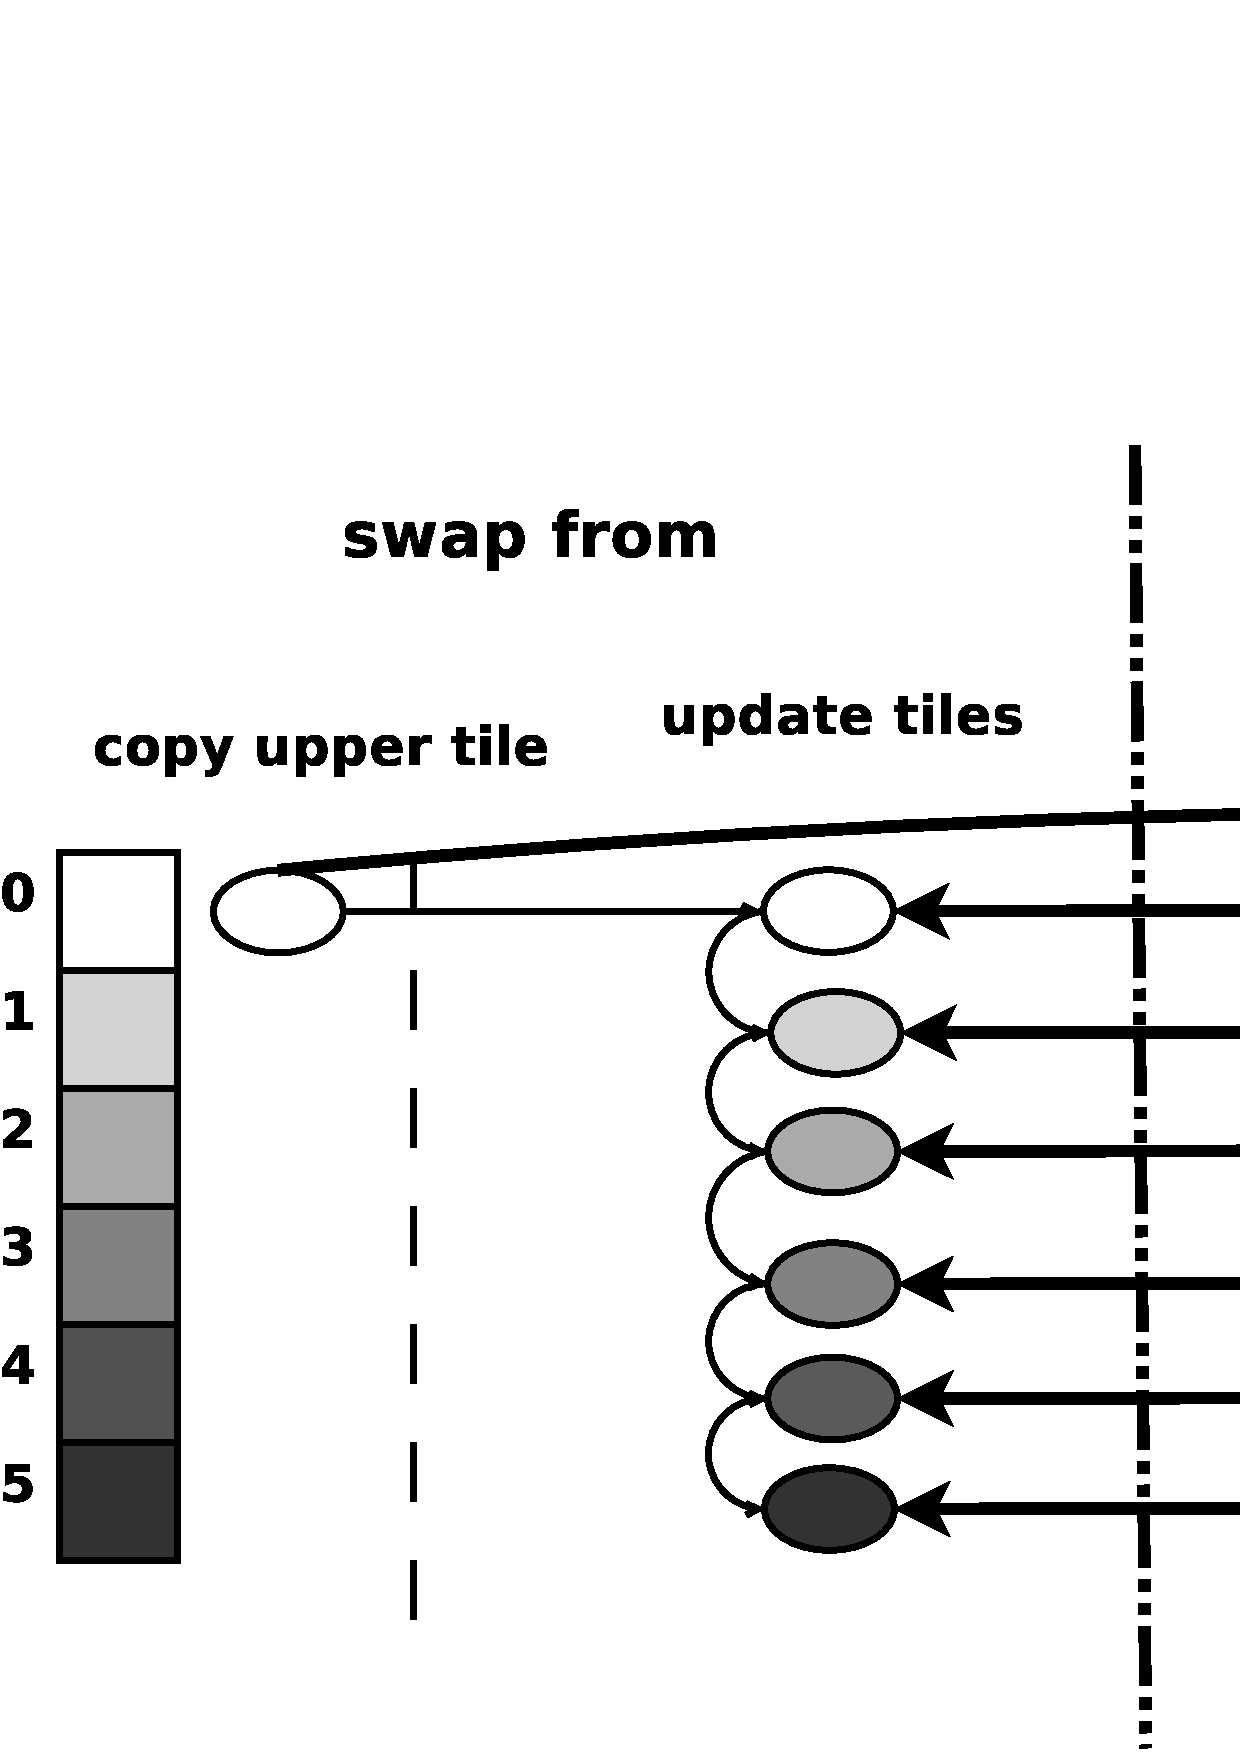
\includegraphics[width=0.8\textwidth]{figures/distributed_update_tf_bw.pdf}
\caption{Swapping operation of update on distributed architecture \label{fig:distributed_update_task_flow}}
\end{taskflow}

As for the panel factorization, we consider that nodes can be multi-core. In order to reduce global communications, each node shares its buffers over its local tiles before to send them to other nodes. Task flow \ref{fig:update_task_flow} shows the update operation for hierarchical architecture. We can see that each node gather first locally the rows moving to the upper tile, before participating to global gather. We also observe that the broadcast can produce a tremendously number of communications, but in fact, the runtime can manage broadcasts operations in order to minimize communications. For that, it can change the DAG of communications to a three, ring or other models of broadcast.

\begin{taskflow}[!ht]
\centering
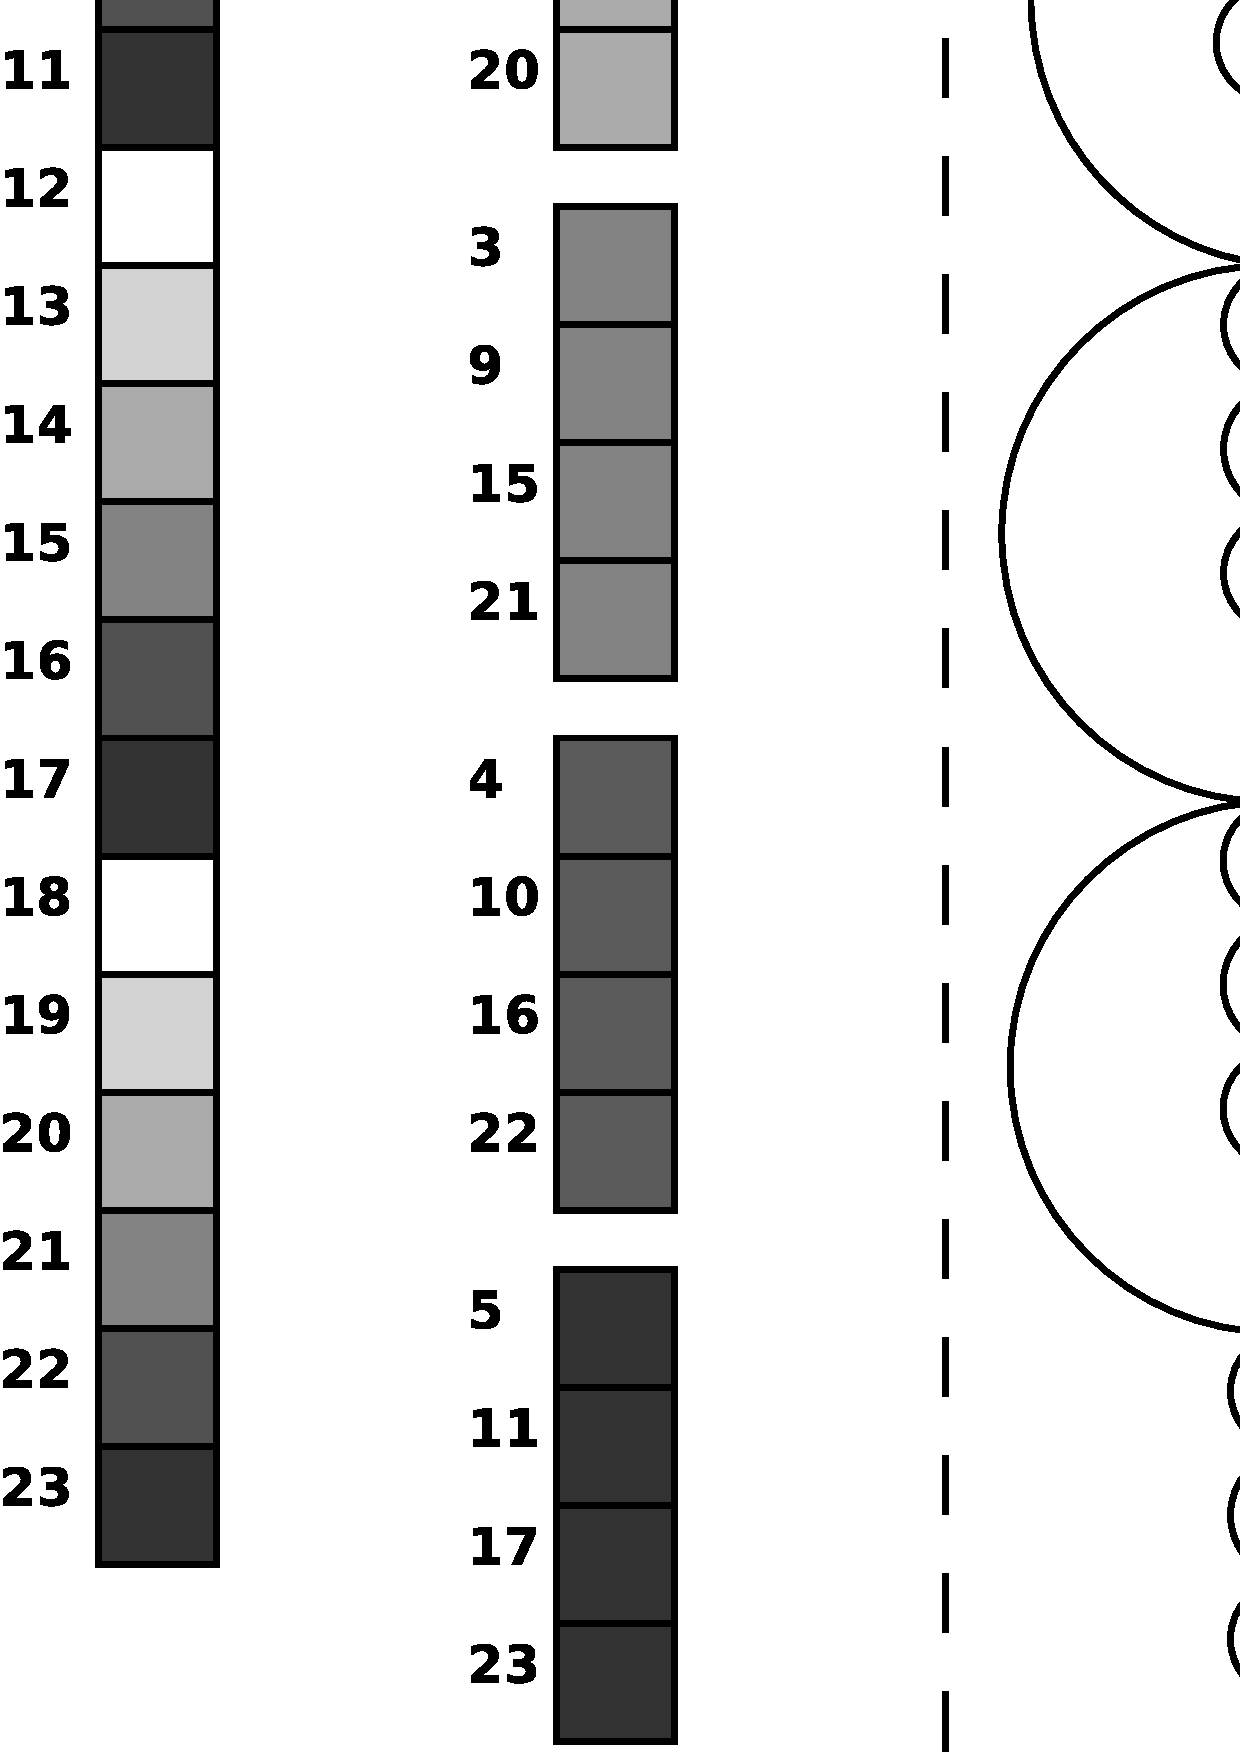
\includegraphics[width=0.8\textwidth]{figures/update_tf_bw.pdf}
\caption{Swapping operation of update on hierarchical architecture \label{fig:update_task_flow}}
\end{taskflow}

Moreover, this update algorithm implemented is a generic solution that can execute update operation after any panel factorization which provides an array of pivots (incremental pivoting, CALU \dots).
